\chapter{Experiment}

In order to validate that the model is accurate for each motion, the torque that causes the device to perform each motion is determined experimentally. The equivalent values produced by the model can be compared with the measured torques to validate the model quantitatively. However, the torque produced by a DC motor cannot be measured or set directly. The torque of a DC motor is proportional to the current running through it, and when the motor isn't moving, the current is proportional to the voltage across the motor terminals. The terminal voltage is varied in this experiment.

\section{Voltage-torque calibration} \label{sec:Voltage-torque calibration}
The relationship between terminal voltage and stalling torque is determined experimentally, this will allow subsequent experiments to measure the terminal voltage and calculate the stalling torque.
To characterise the motors, an experiment was set up to determine the stalling torque produced at different input voltages. In this experiment, the motor lifts a lever with a mass attached. The torque required to lift the lever increases as the lever angle increases, until the motor can no longer provide enough torque and stalls. The lever angle which causes the motor to stall can be used to calculate the stalling torque, specifically by using the horizontal displacement of the mass,
\begin{equation}
	T_\mathrm{Stall} = m g s_x
\end{equation}
where $T_\mathrm{Stall}$ is the stalling torque, $m$ is the mass attached to the lever, $g$ is the gravitational acceleration, and $s_x$ is the horizontal displacement between the mass and the motor axis. The experiment set-up is illustrated in Figure \ref{fig:lever-labelled}.
\begin{figure}[!h]
	\centering
	
\includegraphics[width=0.6\textwidth]{FBDs/lever-labelled}
	\caption{Calibration lever set-up.}
	\label{fig:lever-labelled}
\end{figure}
This test is repeated with different motor voltages.\\

\subsection{Variables}
Independent variable:\\
$\bullet$ Motor voltage (V)\\
Dependent variable:\\
$\bullet$ Distance the weight is lifted (mm)\\
Controlled variables:\\
$\bullet$ Motor used\\
$\bullet$ Lever used\\
$\bullet$ Power supply used\\
$\bullet$ Multimeter used\\
$\bullet$ Ruler used\\

\subsection{Method}

\begin{enumerate}
	\item Remove LIM from motor axle.
	\item Attach the lever to the motor axle.
	\item Measure the weight of the mass on a calibrated scale. \label{stepMeasure}
	\item Drive the motor until the lever is pointing straight down.
	\item Attach the mass to the lever.
	\item Adjust the voltage of the power supply to the chosen value. \label{stepAdjust}
	\item Power on the motor.
	\item Wait until the lever stops moving.
	\item Record the voltage across the motor terminals. 
	\item Quickly power off the motor. Leaving the motor on while stalling can cause damage to the motor.
	\item Measure the horizontal distance that the lever has moved.
	\item Drive the motor until the lever is pointing straight down. \label{stepReset}
	\item Repeat steps \ref{stepAdjust} to \ref{stepReset} with different power supply voltages.
	\item Remove the mass from the lever. \label{stepRemove}
	\item Repeat steps \ref{stepMeasure} to \ref{stepRemove} with different masses.
\end{enumerate}
\subsection{Results}
The measured results, as well as the calculated torque, are shown in Table \ref{voltage-torque-table}, and visualised in Figure \ref{torque-voltage-plot}.

\begin{table}[!ht]
	\centering
	\caption{Recorded results and calculated torque from the calibration experiment.}
	\label{voltage-torque-table}
	\begin{tabular}{|l|l|l|l|}
		\hline
		Mass (g) & Lever (mm) & Voltage (V) & Torque (N$\cdot$m) \\ \hline
		145 & 97 & 0.83 & 0.13797765 \\ \hline
		145 & 101 & 0.92 & 0.14366745 \\ \hline
		145 & 151 & 1.1 & 0.21478995 \\ \hline
		204 & 154 & 1.22 & 0.30819096 \\ \hline
		204 & 229 & 1.56 & 0.45828396 \\ \hline
		542 & 89 & 1.72 & 0.47321478 \\ \hline
		537 & 106 & 1.93 & 0.55840482 \\ \hline
		542 & 106 & 1.8 & 0.56360412 \\ \hline
		537 & 164 & 2.45 & 0.86394708 \\ \hline
		542 & 171 & 2.5 & 0.90921042 \\ \hline
		542 & 220 & 3 & 1.1697444 \\ \hline
		542 & 242 & 3.25 & 1.28671884 \\ \hline
		1289 & 117 & 3.5 & 1.47947553 \\ \hline
		1289 & 136 & 4 & 1.71973224 \\ \hline
		1289 & 160 & 4.5 & 2.0232144 \\ \hline
	\end{tabular}
\end{table}

\begin{figure}[!h]
	\centering
	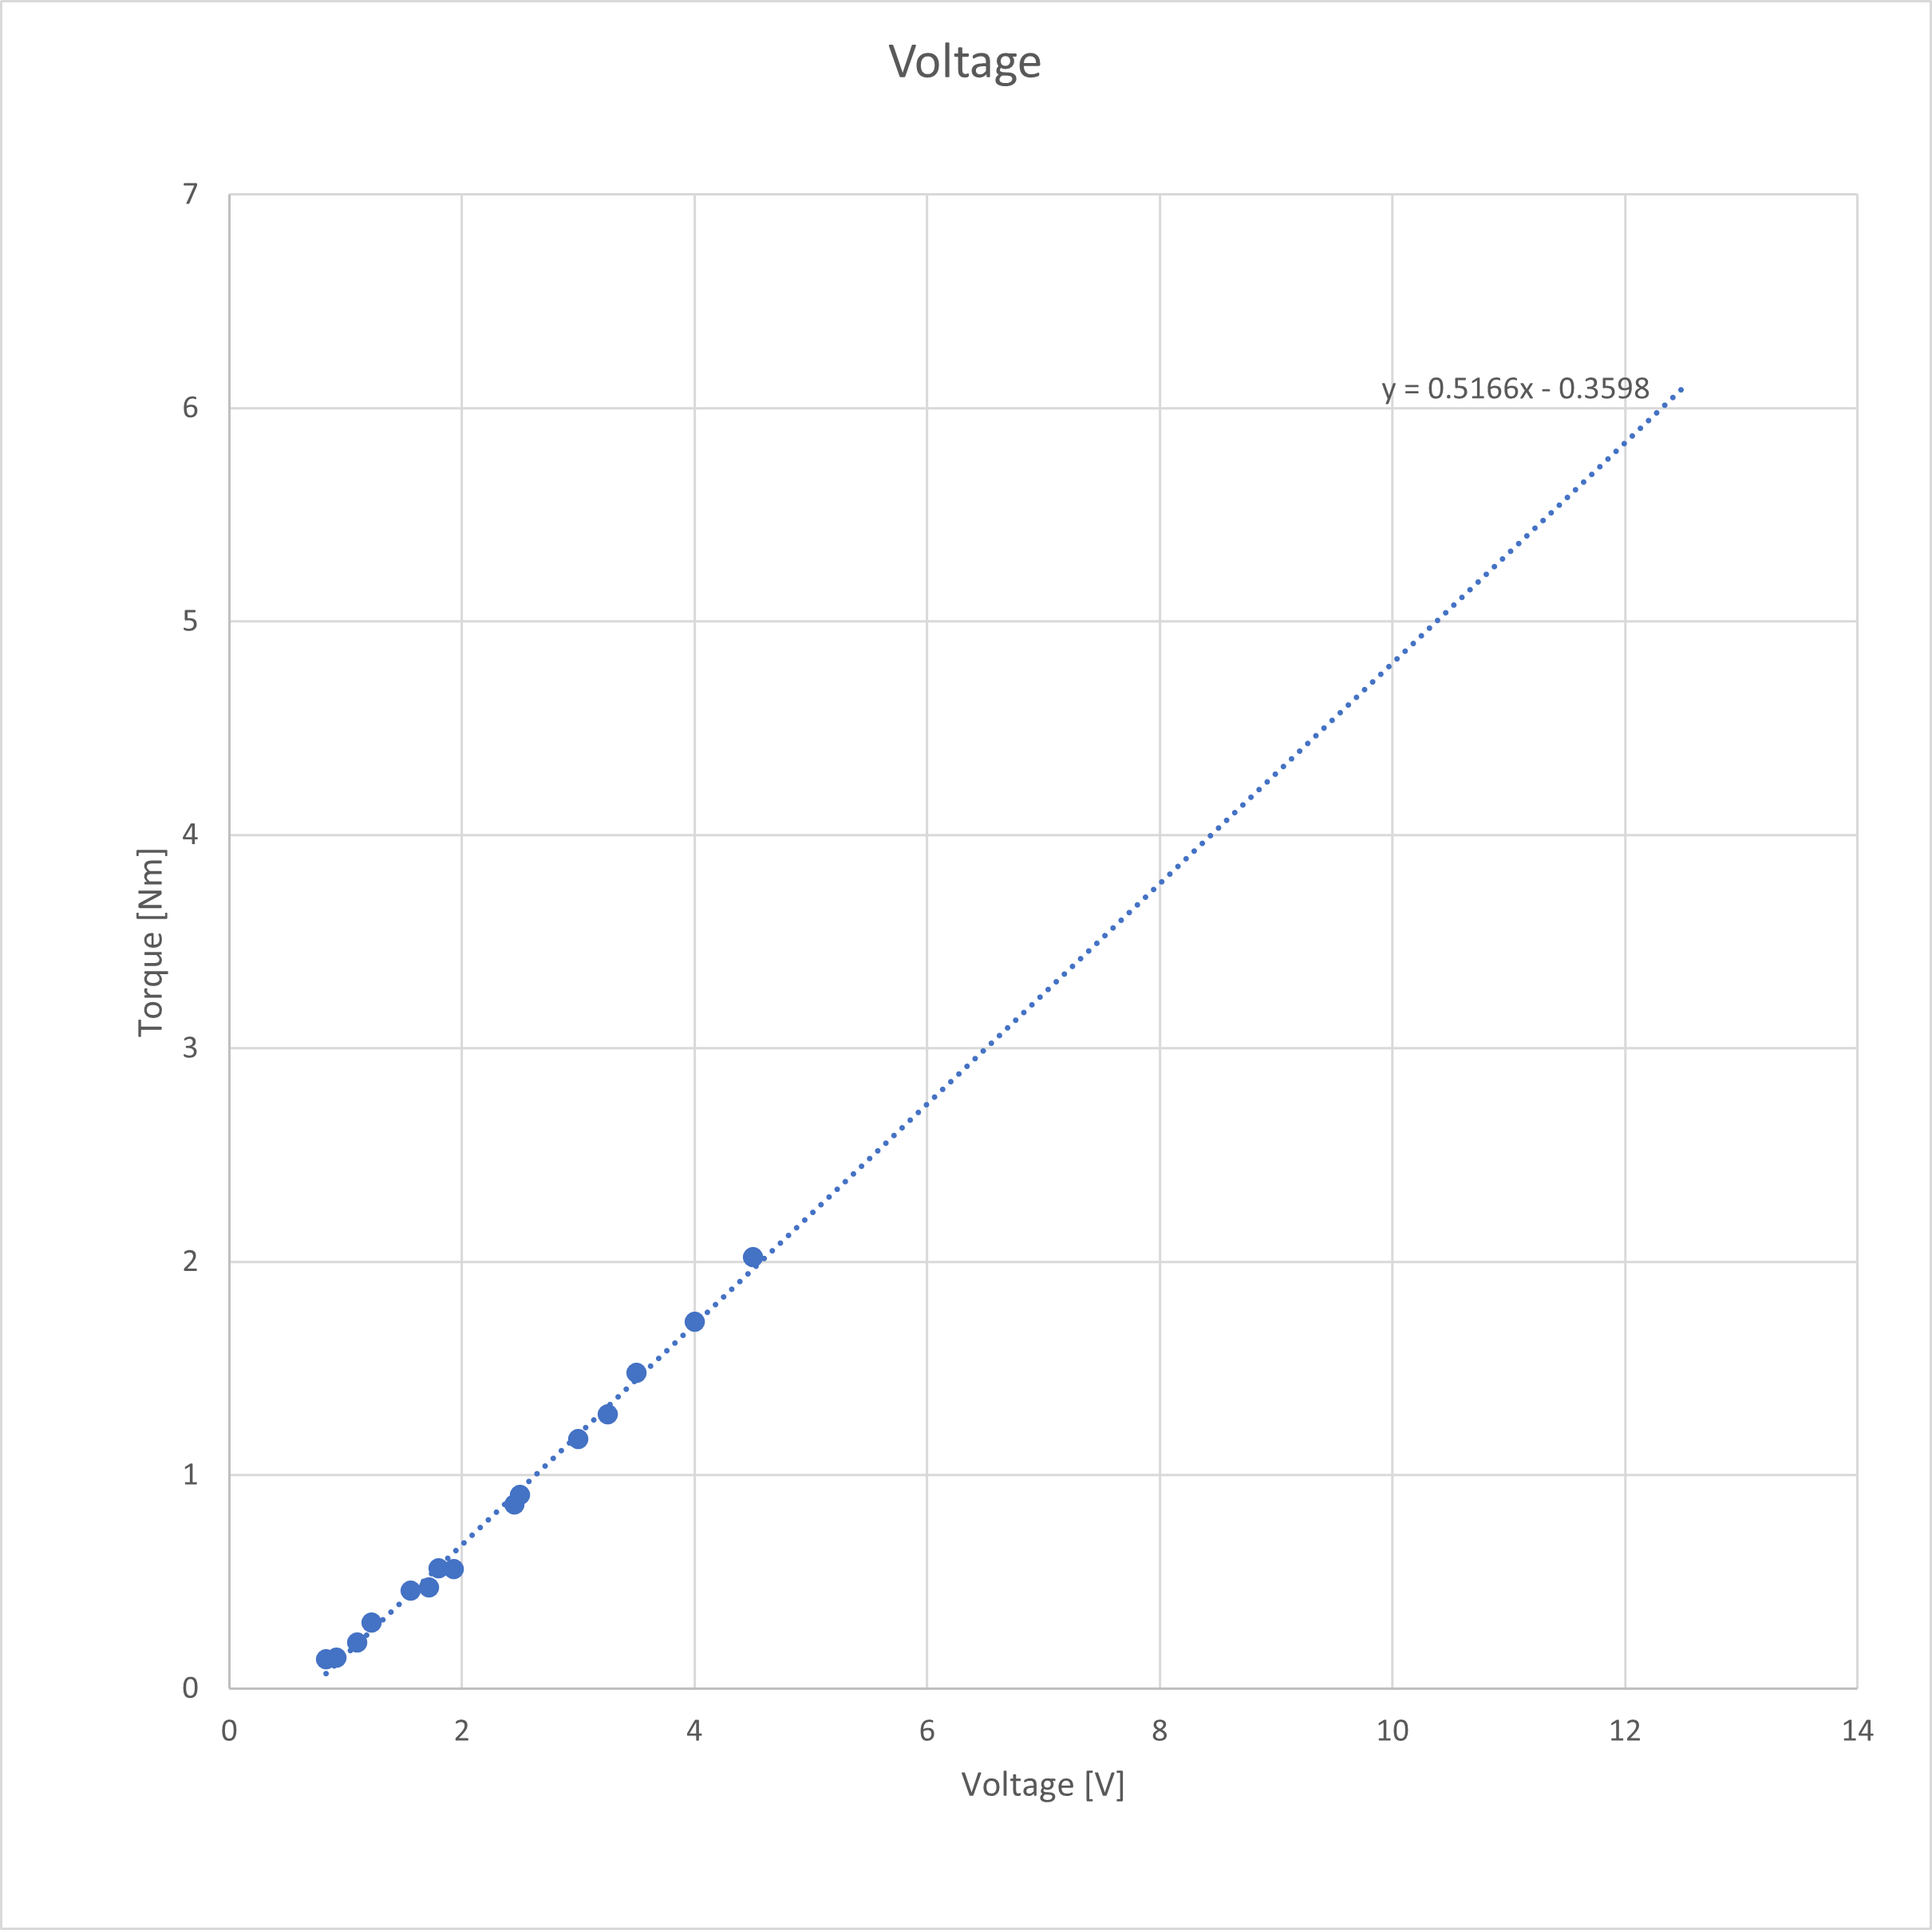
\includegraphics[width=0.8\textwidth]{plots/torque-voltage-relation.png}
	\caption{Relationship between motor voltage and stalling torque.}
	\label{torque-voltage-plot}
\end{figure}

This plot shows a linear relationship between stalling torque and voltage, and gives the formula,
\begin{equation}
	T_\mathrm{Stall} =  0.5166 V - 0.3598 \label{eqTorqueVoltage}
\end{equation}
where $V$ is the motor terminal voltage.
This experiment did not attempt to measure torques beyond 2 N$\cdot$m as this risked damaging the device and was beyond the expected requirements for the device.



\section{Torque measurement}
This experiment aims to determine the torque required to lift the device through each stage of motion. The results of this experiment will be compared with the theoretical required torques provided by the model and the simulation. The device is placed in the starting position for each stage of motion and powered with a certain supply voltage. The motion of the device is then assessed. If the device does not move, the motion is marked as "None"; if the device starts to move but does not complete the stage of motion, it is marked as "Partial"; and if it completes the stage of motion, it is marked as "Full". For this experiment, bricks are stacked to create a staircase with a step height of 10 cm and width of 20 cm. The experimental set-up is shown in Figure \ref{fig:experiment-setup}.\\

\begin{figure}[!h]
	\centering
	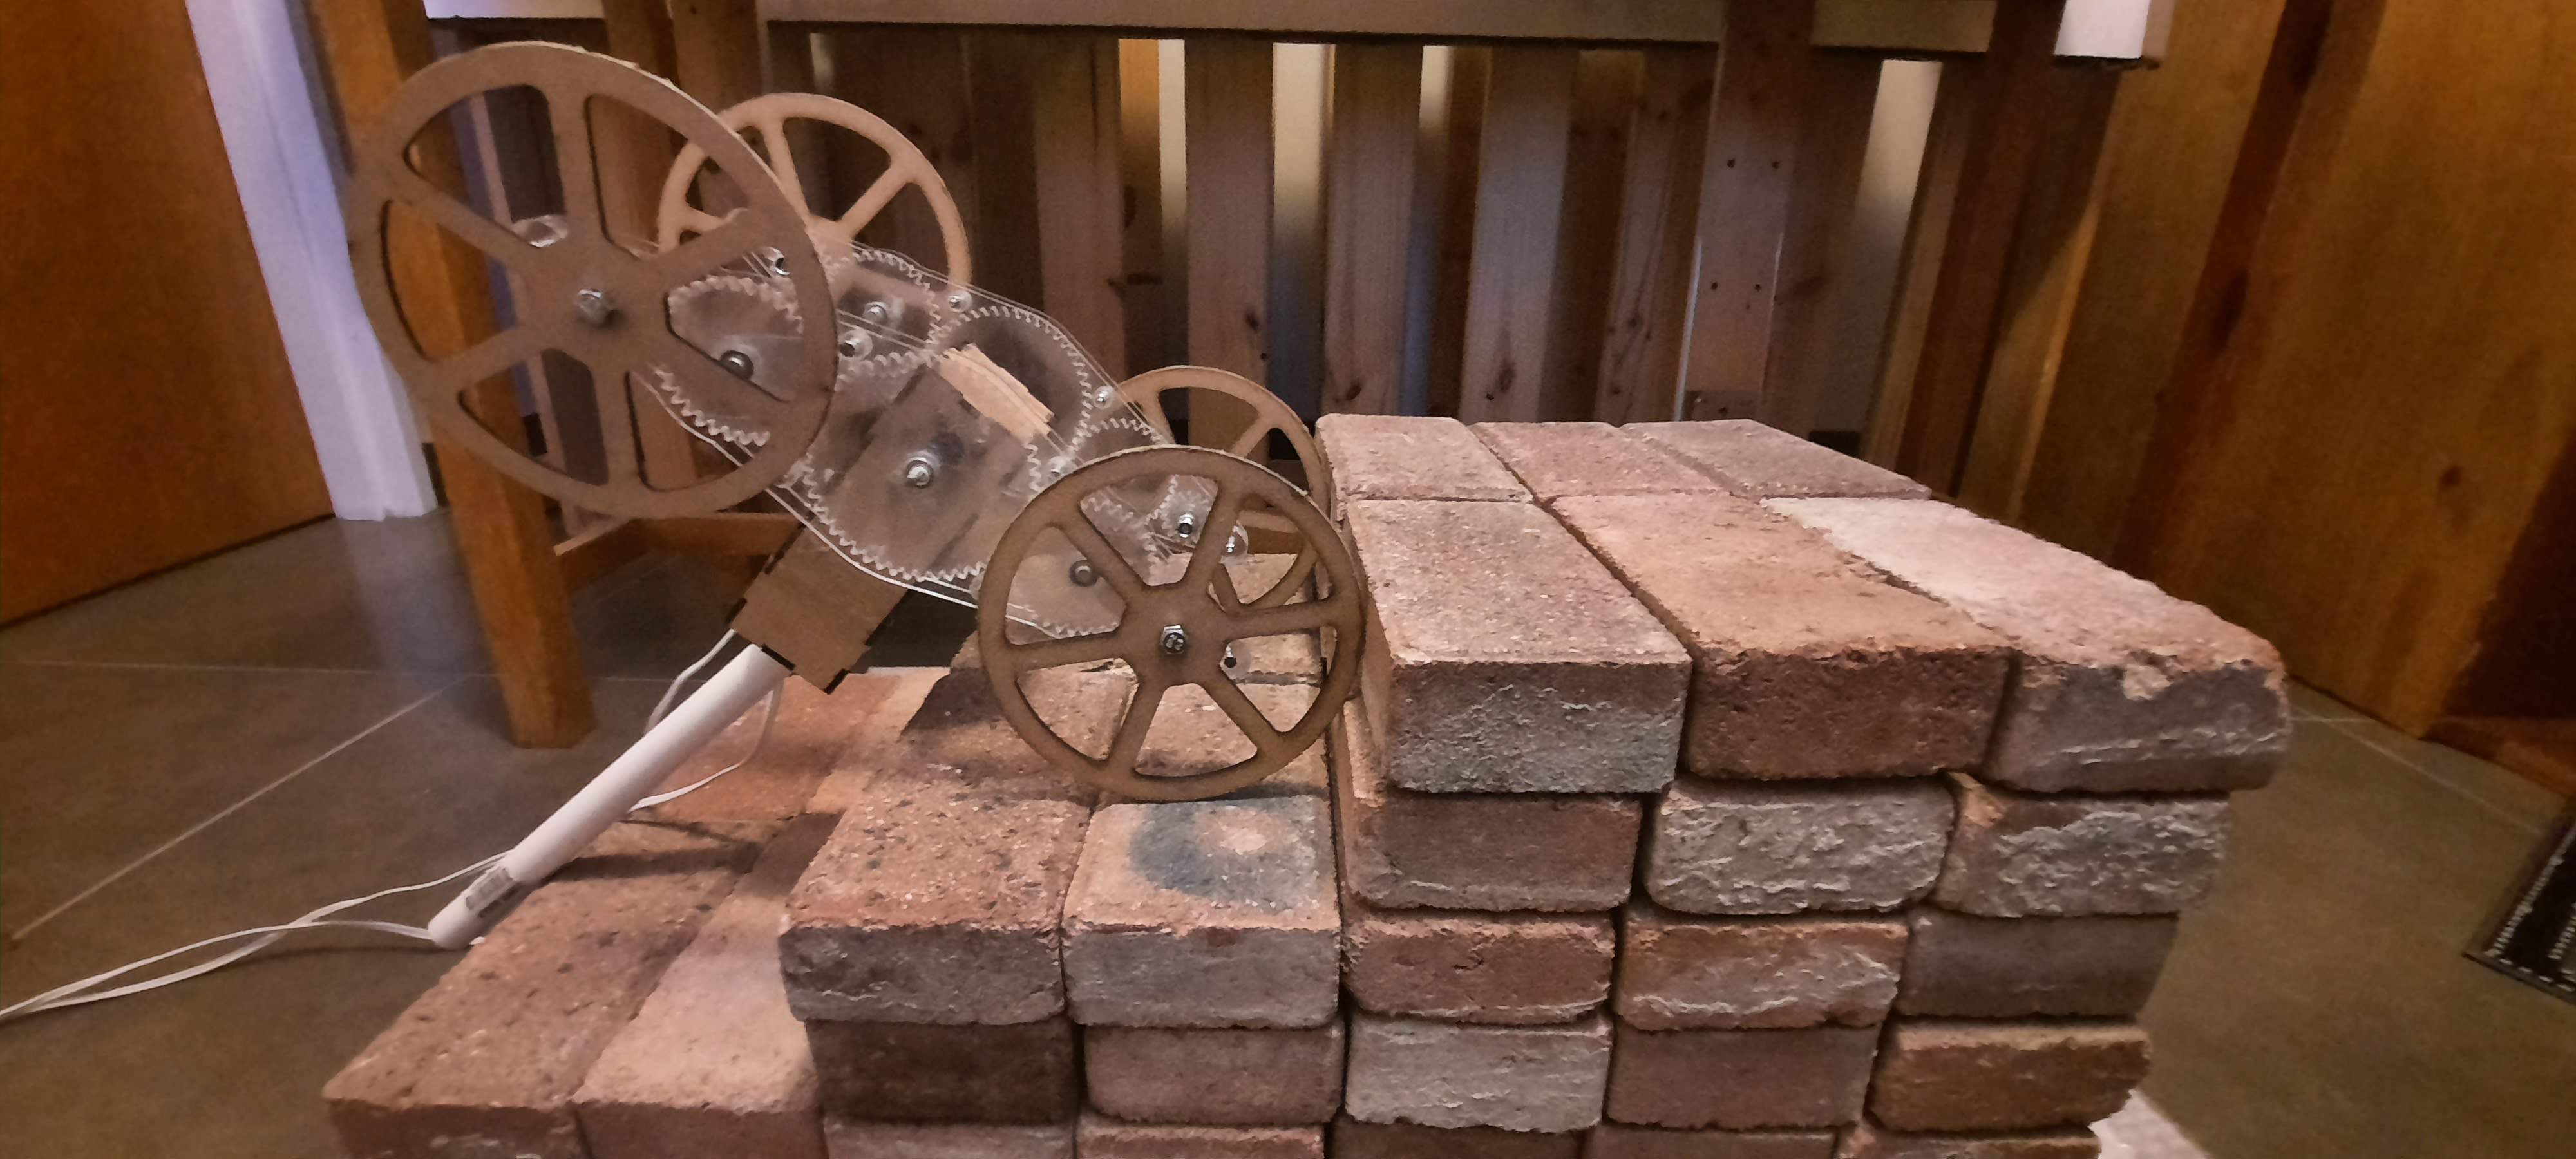
\includegraphics[width=0.8\textwidth]{experiment-setup}
	\caption{Photograph of the experimental set-up, in which the device is performing Stage 4 motion.}
	\label{fig:experiment-setup}
\end{figure}

\subsection{Variables}
Independent variable:\\
$\bullet$ Motor voltage (V)\\
Dependent variable:\\
$\bullet$ Assessment of motion ("Full", "Partial", or "None")\\
Controlled variables:\\
$\bullet$ LIMed device\\
$\bullet$ Stairs\\
$\bullet$ Multimeter used\\


\subsection{Method}

\begin{enumerate}
	\item Place device in the starting position for the chosen stage of motion. \label{stepPlace}
	\item Adjust the voltage of the power supply to the chosen value.
	\item Power on the device.
	\item Observe how the device moves and classify the movement into "Full", "Partial", or "None". 
	\item Record the voltage across the motor terminals. 
	\item Power off the device.\label{stepOff}
	\item Repeat steps \ref{stepPlace} to \ref{stepOff} with a range of power supply voltages.\label{stepRepeatVoltage}
	\item Repeat steps \ref{stepPlace} to \ref{stepRepeatVoltage} for the different stages of motion.
\end{enumerate}

\subsection{Results}

Table \ref{tab:Stage1Torque} shows the measured results for the Stage 1 motion, as well as the torques calculated using Equation \ref{eqTorqueVoltage}. The data for the other stages of motion can be found in Appendix \ref{app:data}.

\begin{table}[!h]
	\centering
	\caption{Torque experiment results for Stage 1}
	\label{tab:Stage1Torque}
	\begin{tabular}{|l|l|l|}
		\hline
		Voltage (V) & Assessment of motion & Torque (N$\cdot$m) \\ \hline
		0.89 & None & 0.099974 \\ \hline
		1.08 & None & 0.198128 \\ \hline
		1.12 & None & 0.218792 \\ \hline
		1.57 & None & 0.451262 \\ \hline
		1.68 & None & 0.508088 \\ \hline
		1.74 & None & 0.539084 \\ \hline
		1.81 & None & 0.575246 \\ \hline
		1.87 & None & 0.606242 \\ \hline
		1.89 & Partial & 0.616574 \\ \hline
		1.98 & Partial & 0.663068 \\ \hline
		2.05 & Partial & 0.69923 \\ \hline
		2.11 & Full & 0.730226 \\ \hline
		2.13 & Full & 0.740558 \\ \hline
		2.25 & Full & 0.80255 \\ \hline
		2.26 & Full & 0.807716 \\ \hline
		2.3 & Full & 0.82838 \\ \hline
	\end{tabular}
\end{table}

This data is plotted in Figure \ref{plotassessment-torque-relation-stage1}, which shows that the full motion only happens with torques of at least 0.73 N$\cdot$m, while partial motion only requires 0.61 N$\cdot$m.

\begin{figure}[h]
	\centering
	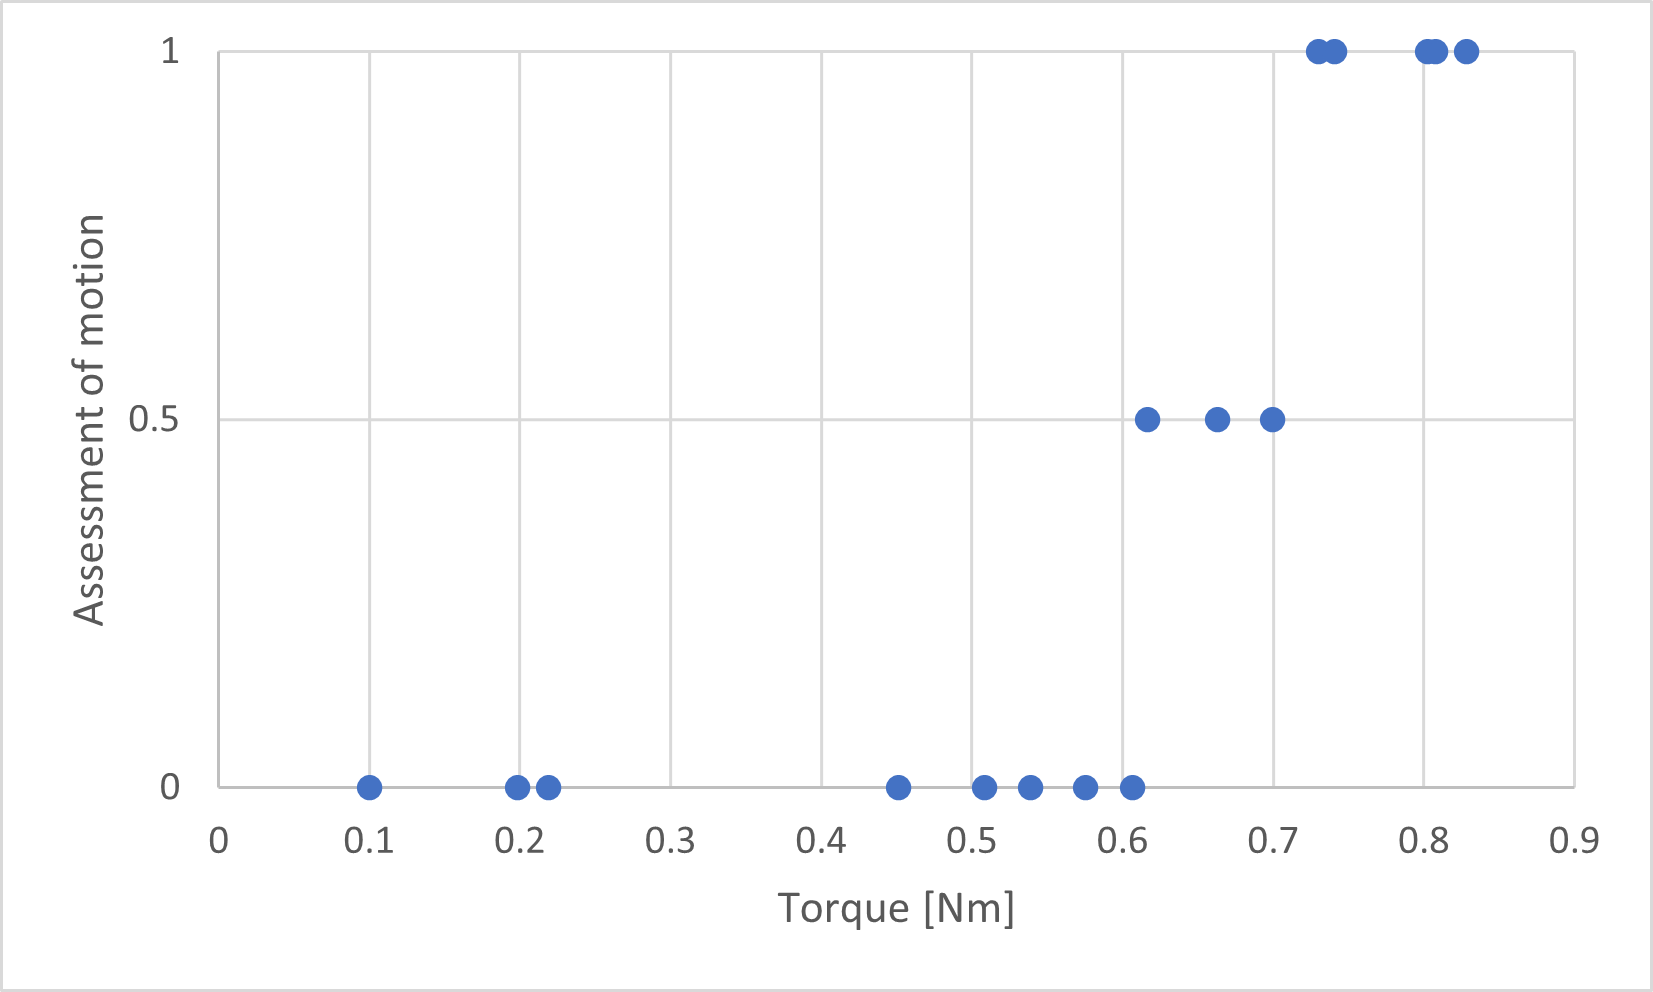
\includegraphics[width=0.8\textwidth]{plots/assessment-torque-relation-stage1}
	\caption{Relationship between torque and motion for Stage 1, with 0, 0.5, and 1 representing "None", "Partial", and "Full" respectively.}
	\label{plotassessment-torque-relation-stage1}
\end{figure}

\section{Current measurement}
This experiment aims to measure the current running through the motors when the LIM climbs steps. Current is proportional to torque in DC motors, so the curve produced by this experiment can be compared with the simulated torque during the same movement. This will allow the kinematic aspects of the model and simulation to be validated, as the stalling torques from the previous experiment can only validate the statics. A 1 $\Omega$ resistor is placed in series with the motor, so that the voltage across the resistor will be equal to the current running through it.\\

\subsection{Variables}
Independent variable:\\
$\bullet$ Time (s)\\
Dependent variable:\\
$\bullet$ Current (A)\\
Controlled variables:\\
$\bullet$ LIM device used\\
$\bullet$ Power supply used\\
$\bullet$ Oscilloscope used\\
$\bullet$ Oscilloscope probes used\\
$\bullet$ Resistor used\\

\subsection{Method}

\begin{enumerate}
	\item Connect a 1 $\Omega$ resistor in series with one motor.
	\item Attach the oscilloscope probe to either end of the resistor.
	\item Configure the oscilloscope trigger on a rising edge with a 5 second period.
	\item Place the device against a step or wall so that it will perform Stage 1 motion when powered.
	\item Power on the device until it has completed stage 1 motion.
	\item Record the voltage data from the oscilloscope.
\end{enumerate}

\subsection{Results}

Figure \ref{fig:current-stage-1} shows the plot recorded by the oscilloscope. It shows that there is a large spike in current as the device powers on, followed by a fairly constant but noisy current until a slight dip at 2.7 s, then a drop when it completes stage 1 at 3.25 s. The spike at the start is due the motor producing no counter-electromotive force (EMF) when it is stationary. As the motor shaft initially accelerates, the current rapidly drops due to the counter-EMF produced by the motor. The noise shown in the plot can be attributed to the constant switching of the brushed DC motor. The noise could be eliminated by implementing a low pass filter, but this would also filter out the initial spike. 
\begin{figure}[h]
	\centering
	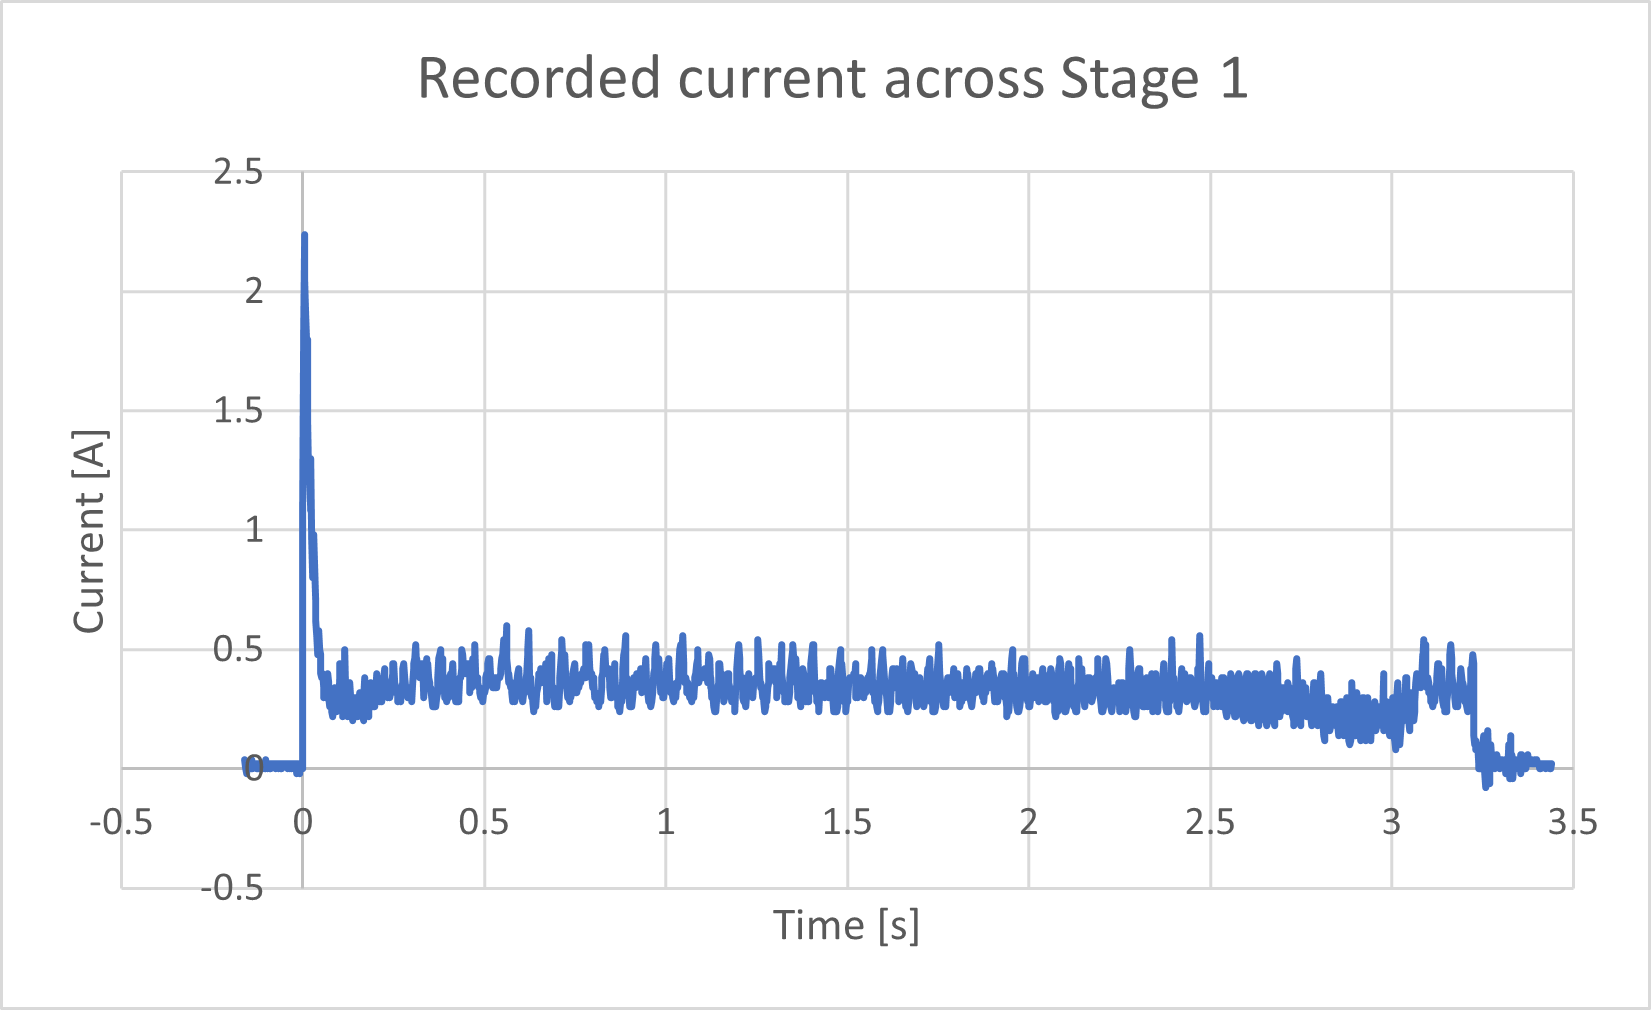
\includegraphics[width=0.8\textwidth]{plots/current-stage-1}
	\caption{Current recorded over time as the device completes Stage 1}
	\label{fig:current-stage-1}
\end{figure}